\documentclass[a4paper, 12pt]{article}

\usepackage[utf8]{inputenc}
\usepackage{latexsym,amsfonts,amssymb,amsthm,amsmath}
\usepackage{setspace}
\usepackage{physics}
\usepackage{graphicx}
\usepackage{newtxtext}
\usepackage{extsizes}
\setlength{\parindent}{0in}
\setlength{\oddsidemargin}{0in}
\setlength{\textwidth}{6.5in}
\setlength{\textheight}{8.8in}
\setlength{\topmargin}{0in}
\setlength{\headheight}{8pt}

\onehalfspacing


\title{
  \vspace{-1.5cm}
  \textbf{Probability model of random sample.\\ Central Limit Theorem}
  \vspace{-1.5cm}
}
\date{}

\begin{document}

\maketitle


\section{Mathematical statistics as a science}

Mathematical statistics is a science that deals with data - their collection, analysis, representation, interpretation and making appropriate conclusions that are scientifically based.\\

It is applied in many academic disciplines from natural and social sciences to humanities. It also finds great application in industry, in solving many practical tasks.\\

\subsection{Data}

Statistical data are characteristics (or information) gathered by observing or studying uniform objects. For example, on the set of all children in Skopje at the age of ten, the following characteristics can be examined: height, weight, success at school, gender, nationality, eye color, etc. On FINKI's set of computers, one can examine the characteristics: processor speed, RAM size, disk capacity, etc.

\subsection{Population and feature}

In statistics, a set of uniform objects or results of an operation, which have one or more common characteristics, is called a population. The common characteristic is called a feature. \\

The population is denoted by $\Omega$, because it is the set of all possible outcomes regarding an experiment (the set of elementary events).


\subsection{Examples}

Let us consider the population ”children in Skopje”. We can observe different
characteristics for of the children: height, weight, success, gender, nationality, eye
color, etc. - these are only few of the features for this population. \\

For the population ”computers of FINKI”, the features are: processor speed, size of
RAM, disk capacity, etc.\\

The value obtained by the feature is variable value and it cannot be reliably
predicted for a specific individual from the population. Therefore, we will consider
each feature to be a random variable.\\

In statistics we work with data collected for different features.

\subsection{Types of data}

\begin{itemize}
  \item \textbf{Numerical}: discrete or continuous (interval data)
  \item \textbf{Categorical}: nominal or ordinal
\end{itemize}

\subsubsection{Numerical data}

\textbf{Numerical data} is data that is expressed in numbers. This data is related to specific measurements (such as measuring a person's height, weight, IQ, or blood pressure) or is related to counts (such as the number of shares owned by a person, number of students in one group, etc.). Numerical data are also called quantitative data. \\

Numerical data can be further divided into two types: \textbf{discrete} and \textbf{continuous}.\\ 

\textbf{Discrete data} is obtained as a result of counting. The set of possible values for this data may be finite or countable. For example, the number of heads in 100 tosses of a coin can take a value from 0 to 100 (finite case), but the number of tosses until 100 heads are got can take a value from 100 to infinity (countable case).\\

\textbf{Continuous data} is obtained by measurements. Their possible values can only be described using intervals on the real scale. For example, the working time of a machine is in the interval $[0,T]$, where T is the maximum working life of the machine, and it can be infinity. Hence, this data is from an infinite uncountable set.

\subsubsection{Categorical data}

\textbf{Categorical data} represent characteristics such as gender, nationality, eye color, marital status, hometown, etc. Categorical data may be assigned with numerical values (for example, "1" to indicate male and "2" to indicate female), but those numbers have no mathematical meaning. Categorical data are also called qualitative data.

Categorical data can be \textbf{nominal} or \textbf{ordinal}.

\subsubsection{Nominal data}
Nominal values represent discrete units and are used to mark (label) the variables and
they have no quantitative value. Numbers representing data can only be used to classify or categorize. For example, employee identification numbers (or index numbers) are nominal data. Some other types of characteristics that often provide nominal level data are gender, religion, ethnicity, geographic location, and place of birth. It can be seen that nominal data has no order. Therefore, if you were to change the order of its values, the meaning would not change.

\subsubsection{Ordinal data}

Ordinal data can be used for ranking or ordering. For example, a supervisor might rate
three employees by ranking their productivity with numbers from 1 to 3 (most
productive, least productive, and somewhere in between). But it cannot say that the
differences in productivity between workers ranked 1 and 2; and by 2 and 3 are
necessarily the same, i.e., the distances represented by consecutive numbers are not
always equal. An ordinal scale is usually used to measure non-numerical characteristics such as happiness, customer satisfaction, etc.


\section{Goal of statistics}

Most often, when solving practical problems, the distribution of the feature is not known in advance. Hence, the aim of statistics is to determine that distribution by using certain methods, or to find its characteristics, to evaluate some parameters, etc.

\subsection{Types of features}

Depending on the values (type of data) they can receive, the features can be numerical
(quantitative) or categorical (qualitative). Numerical features can be discrete and
continuous, as can random variables.

\subsection{Sample}


Most often, when performing statistical tests, it is impossible to examine all elements of the population. It happens that the examinations last a long time, are associated with the expenditure of large financial resources or even more, during the examination of certain objects, their destruction occurs. Therefore, a part of the population is selected on which all the tests are carried out and conclusions should be made that will apply to the entire population with a certain probability.

The part of the population on which the necessary tests are carried out is called a
\textbf{sample}. The number of elements in the sample is called the \textbf{sample size}.

\subsubsection{Choice of the sample}

The conclusions drawn on the basis of the sample should be valid for the entire
population. To achieve this, it is necessary that the sample be representative, i.e. to represent a mini-model of the population. To achieve this, it is necessary that every element of the population has an equal chance of entering the sample. So, the selection of each element \textbf{should be independent and random}.

\subsubsection{US Elections Example and Analysis}

Deviation from the principle of random selection can lead to serious errors. Let’s
consider the following real-life example. The American magazine ”Literary Digest”
conducted a survey to examine the public opinion about the upcoming presidential
elections in the USA in 1936. The candidates were F. Roosevelt and A. Landon. To
select a sample, the magazine used a telephone directory, magazine subscribers, lists of members of some clubs. 10 million addresses were selected and a survey with questions about the candidates was sent to all of them. The magazine spent a lot of money on sending the cards and processing the data. Responses were received from 2.4 million voters. It was announced that A. Landon is the elected president. The result of the election (F. Roosevelt won) confirmed that the forecast was wrong. \\

What went wrong? In this case, two errors were made. First, during that period of reign of economic crisis, only the richest had phones. Second, the survey was mostly answered by business people, who, in fact, had a habit of answering letters, and all of them supported Landon. On the other hand, two sociologists, regarding the same question, conducted a survey with 50 thousand respondents and came to the right answer. The reason for that is that they not only chose the sample correctly, but started from the fact that society is made up of different social layers and most of the members of one layer support the same candidate. Thus, with the help of the study by social layers, conclusions were made that are valid for the entire country.

\section{Random sample}

For a given population, suppose we observe the feature $X$. Let $X_1$ be the value of $X$ observed in the first run of the experiment, let $X_2$ be the second observed value etc., let $X_n$ the value observed in the n-th run of the experiment. These random variables $X_1, X_2, \dots ,X_n$ have the same distribution as the feature $X$, i.e. they are equally distributed and independent. \\

\textbf{Definition 1.} The random vector $(X_1, X_2, \dots ,X_n)$ is a random sample for the feature $X$, if $X_1, X_2, \dots,X_n$ are independent random variables and all $X_i$ have the same distribution as the feature $X$.\\


\subsection{Random sample realization}

When the random variables $X_1, X_2, \dots ,X_n$ get concrete values from the population, then one realization of the random sample is obtained.\\

For example, let $(X_1, X_2, X_3, X_4, X_5)$ be a random sample of size 5 for the feature $X$ - height of FINKI students. If $5$ such students are randomly selected and their height is measured, then one realization of the sample will be obtained. For example, $(192, 184, 170, 185, 190)$ is one realization of the sample, $(187, 190, 167, 178, 194)$ is another concrete realization of the sample based on 5 other random choices, and so on.\\

\textbf{Definition 2.} The set $W \subseteq R$ $n$ of every possible realizations $(x_1, x_2, \dots , x_n)$ of the random sample with size $n$ is called sample data space.\\


\subsection{Empirical random sample distribution}

\textbf{Definition 3.} Let $(X_1, X_2, \dots ,X_n)$ be a random sample of feature $X$. The function

\[ F_n(X) = \frac{\text{number of elements in the sample space that are $<$ x}}{n} = \frac{1}{n}\sum_{i=1}^{n}I_{\{ X_i<x \}} \]

is called \textbf{empirical distribution of X.}\\

Here, $I_{\{Xi<x\}}$ is indicator of the event $\{X_i < x\}$ - it will be 1, whenever $X_i < x$. Thus we will sum as many 1s as there are elements in the sample that are smaller than the given $x$. The graph of this function has a stairs shape with jumps of height $1/n$ in each of the n-th data in the sample.





\subsection{Empirical random sample distribution}

It is shown that as $n$ increases, the empirical distribution function of $X$ increasingly approaches the distribution function of the feature $X$.\\ 

Practically, when $n\rightarrow +\infty$ the empirical distribution of $X$ tends t othe true distribution of the feature $X$.\\


On the graphs, the empirical distribution function of $X$ is represented by a black line, and the distribution function of the feature $X$ by a red line.\\

Thus, the bigger sample we have, the closer we are to the real distribution of $X$.


\section{Statistics}

A number of methods in statistics use sample functions that are also random variables. We will call those functions \textbf{statistics}.\\

\textbf{Definition 4.} A function of the random sample $(X_1, X_2, \dots ,X_n)$ for the feature $X$, which is itself a random variable, is called a statistic.

At a specific realization $(x_1, x_2, \dots , x_n)$ of the sample, the statistic will get one specific value, which we will call the \textbf{realization of the statistic}.

\subsection{Example}

Exampe 1. Let $(X_1, X_2, X_3, X_4, X_5)$ be a random sample with size 5 for the feature $X$ - height of FINKI students. Then the function

\[ U = \frac{X_1 + X_2 + X_3 + X_4 + X_5}{5} \]

is one function of the sample, which itself is a random variable, i.e. $U$ is a statistic. If one realization of the sample is taken, for example, $(192, 184, 170, 185, 189)$ then one value (realization) of the statistic $U$ is obtained: 

\[ U = \frac{192+184+170+185+189}{5} = 184 \]

Another choice of $5$ students will give us another realization of the random sample and with that, another values of the random variable $U$.

\section{Important statistics}

If $(X_1, X_2, \dots ,X_n)$ is a random sample of size $n$, we can define various statistics, among which the more famous are:

\begin{itemize}
  \item Average or arithmetic mean
  \item Sample variance (dispersion) and standard deviation
  \item Moments of a random sample
  \item Ordered statistics
  \item Median
  \item Range etc.
\end{itemize}

\section{The Sample mean. CLT and Normal Distribution}

\subsection{Average (Arithmetic Mean)}

Let $(X_1, X_2, \dots ,X_n)$ be a random sample for the random variable $X$ which has a mean $\mu$ and variance $\sigma^2$. This means that the random variables $X_1, X_2, \dots ,X_n$ are independent and equally distributed random variables with mean $\mu$ and variance $\sigma^2$. Let $\displaystyle\sum_{i=1}^{n}X_i$ be their sum.\\

\textbf{Definition 5.} The average (or arithmetic mean) of the sample $X_1, X_2, \dots, X_n$ is defined by

\[ \overline{X} = \frac{1}{n}\sum_{i=1}^{n}X_i \]

\subsection{Random sample average properties}

\textbf{Theorem 1:} If $X$ is a random variable with mean $EX = \mu$ and variance $DX = \sigma^2$ and $(X_1, X_2, \dots ,X_n)$ is a random sample for that random variable, then

\[ E\overline{X} = \mu, \quad \quad D\overline{X} = \frac{\sigma^2}{n} \]


\textbf{Proof:} From $EX_i = \mu$ and $DX_i=\sigma^2$, for $i=1,2,\dots,n$ we get:


\[ E\overline{X} = E\left( \frac{1}{n}\sum_{i=1}^{n}EX_i \right) = \frac{1}{n}\sum_{i=1}^{n}EX_i = \frac{1}{n}\sum_{i=1}^{n}\mu = \frac{n\mu}{n} = \mu  \]

while for the variance, due to the independence of $X_i$ and $X_j$ for $i\neq j$, we get:

\[ D\overline{X} = D\left( \frac{1}{n}\sum_{i=1}^{n}EX_i \right) = \frac{1}{n^2}\sum_{i=1}^{n}DX_i  = \frac{1}{n^2}\sum_{i=1}^{n}\sigma^2 = \frac{n\sigma^2}{n^2} = \frac{\sigma^2}{n} \]



\newpage
\section{Central limit theorem}

One of the most significant results in probability and statistics is the central limit
theorem which further emphasizes the importance of the normal distribution. According
to this theorem, if one takes a sum of a large number of independent and equally distributed random variables (regardless of their distribution), the sum will have an
approximately normal distribution. The same holds for the average (arithmetic mean) of
a large number of independent and equally distributed random variables (regardless of
their distribution).\\

Therefore, the normal distribution is one of the most common distributions of real
quantities. Characteristics such as: height, weight of people, most often, have a normal distribution. Also, errors made during measurements in physics, chemistry, etc. have a normal distribution.\\

\textbf{Theorem 2. Central limit theorem.} Let $X_1, X_2, \dots ,X_n$ be independent and equally distributed random variables with mean $\mu$ and dispersion $\sigma^2$. If $n$ is large enough then:

\begin{itemize}
  \item the sum $\displaystyle\sum_{i=1}^{n}X_i$ has approximately normal distribution with mean $n\mu$ and dispersion $n\sigma^2$ i.e. $\displaystyle\sum_{i=1}^{n}X_i \sim \mathcal{N}(n\mu, n\sigma^2)$
  \item the mean $\displaystyle\overline{X}\frac{1}{n}\sum_{i=1}^{n}X_i$ has approximately normal distribution with mean $\mu$ and dispersion $\displaystyle\frac{\sigma^2}{n}$ i.e. $\displaystyle\overline{X} \sim \mathcal{N}(\mu, \frac{\sigma^2}{n})$
\end{itemize}

The Central Limit Theorem gives the asymptotic distribution of the sample sum and the sample mean $\overline{X}$ when  $n \rightarrow \infty$. This approximation is relatively good for $n\geq30$ and is getting better as $n$ increases. \\

The central limit theorem is illustrated with the following example. Let $X$ be the average of the values got with tossing of n dices. For $n = 1, 2, 3, 5, 10$, distributions are got.

\begin{figure}[h]
  \centering
  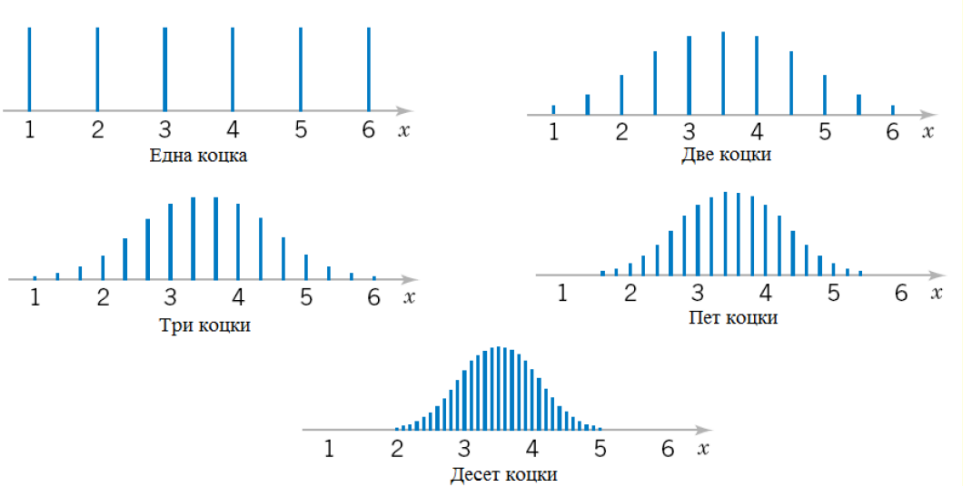
\includegraphics[width=0.6\textwidth]{image.png}
  \caption{}
  \label{fig:clt_1}
\end{figure}

From the previous figure it can be seen that the shape of the distribution is very close to the shape of a normal distribution, even for $n = 3,\ n = 5$.\\

But, we need to realize that the distribution of averages is discrete, and the normal
distribution is of absolutely-continuous type. Hence, the approximation will be better, if n is larger. From many practical examples, it has been concluded for various distributions that if $n > 30$, the approximation with a normal distribution can be considered good enough.\\

From the central limit theorem, with standardization we get

\[ \frac{\sum_{i=1}^{n} X_i - n\mu }{\sqrt{n\sigma^2}} = \frac{\sum_{i=1}^{n} X_i - n\mu }{\sigma \sqrt{n}} = \frac{\overline{X} - \mu}{\frac{\sigma}{\sqrt{n}}} \sim N(0,1) \]

Thus the probability

\[  P\left( \frac{\sum_{i=1}^{n} X_i - n\mu }{\sqrt{n\sigma^2}} < x \right) 
= P\left( \frac{\overline{X} - \mu}{\frac{\sigma}{\sqrt{n}}}  \right) \approx \Phi(x) \]


i.e. it is approximated with the value of the cdf of standard normal distribution in the value $x$, i.e. $\Phi(x)$. The values for $\Phi(x)$ can be read from tables for standard normal distribution or calculated with \texttt{R}.


\subsection{Example with CLT}

\subsubsection{Example}

On a hard disk there is free space of $330MB$. Is that enough space for storing $300$ independent figures, if each figure has expected size of $1MB$ with dispersion of $0.25MB$?

\subsubsection{Example}

Let $X_1, X_2, \dots ,X_{36}$ be independent and equally distributed random
variables with mean $\mu = 8$ and dispersion $\sigma^2 = 9$. Find the probability that the average of these random variables is between $7.8$ and $8.2$.


\subsection{Determining the z value}

How to determine for which value of z, $\Phi(z) = 0.2$ for the random variable
$Z \sim N(0, 1)$? In the table with values of $\Phi$ the value $0.2$ is searched (or some values closest to it) and then it is read for which value of z, $\Phi(z) = 0.2$. From the table $z = -0.84$ is read. $20\%$ of the area is before $z = -0.84$\\

Suppose that $X\sim N(\mu, \sigma^2)$ and we want to compute $P(a<X<b)$. We know that $\displaystyle \frac{X-\mu}{\sigma} = Z \sim N(0,1)$ so we will use this transformation and we will read from a table for standardized normal distribution. With the transformation the following holds:

\begin{align*}
  P\{ a<X<b \}  &= P\{ \frac{a-\mu}{\sigma} < \frac{X-\mu}{\sigma} < \frac{b-\mu}{\sigma} \} \\
  &= P\{ \frac{a-\mu}{\sigma} < Z < \frac{b-\mu}{\sigma} \}\\
  &= F_Z\left( \frac{b-\mu}{\sigma} \right) - F_Z\left( \frac{a-\mu}{\sigma} \right)\\
  &= \Phi\left( \frac{b-\mu}{\sigma} \right) - \Phi\left( \frac{a-\mu}{\sigma} \right)
\end{align*}

Now the vaues $\Phi\left( \frac{b-\mu}{\sigma} \right)$ and $\Phi\left( \frac{a-\mu}{\sigma} \right)$ are read separately from a table for standardized normal distribution.


\newpage
\section{Sample variance}

Let $(X_1, X_2, \dots ,X_n)$ be a random sample for the random variable $X$ which has a mean $\mu$ and variance $\sigma^2$. This means that the random variables $X_1, X_2, \dots,X_n$ are independent and equally distributed random variables with mean $\mu$ and variance $\sigma^2$.\\

\textbf{Definition 6.} The sample variance is defined by

\[ s^2 = \frac{1}{n-1}\sum_{i=1}^{n}(X_i - \overline{X})^2 \]

and the sample standard deviation with $s=\sqrt{s^2}$\\

\textbf{Theorem 3.} The variance $s^2$ of the random sample with size $n$ can be written in the form:

\[ s^2 = \frac{\sum_{i=1}^{n} X_i^2-n\overline{X}^2}{n-1} \]

\textbf{Proof:}

\begin{align*}
  s^2 &=  \frac{1}{n-1}\sum_{i=1}^{n}(X_i - \overline{X})^2\\
  &= \frac{1}{n-1}\sum_{i=1}^{n}( X_i^2 - 2\overline{X}X_i + \overline{X}^2 )^2 \\
  &= \frac{1}{n-1}\sum_{i=1}^{n}X_i^2 - 2\overline{X}\sum_{i=1}^{n}X_i+n\overline{X}^2 \\
  &= \frac{1}{n-1}\sum_{i=1}^{n}X_i^2-2\overline{X}\cdot n\overline{X}+n\overline{X}^2 \\
  &=  \frac{\sum_{i=1}^{n} X_i^2-n\overline{X}^2}{n-1}\\
\end{align*}

This form is used more often, since it is easier for calculation.\\

\textbf{Theorem 4:} If $X$ is a random variable with mean $EX=\mu$ and variance $DX=\sigma^2$ and $\left( X_1,X_2,\dots,X_n \right)$ is a random sample for that random variable then

\[ ES^2=\sigma^2 \]

\textbf{Proof.}

\begin{align*}
  ES^2 &= E\left( \frac{\sum_{i=1}^{n} X_i^2-n\overline{X}^2}{n-1} \right) \\
  &= \frac{1}{n-1} \sum_{i=1}^{n} E(X_i^2)-nE(\overline{X}^2) \\
  &= \frac{1}{n-1} [ n(\sigma^2+\mu^2) - n(\frac{\sigma^2}{n}+\mu^2) ] \\
  &= \frac{1}{n-1} (n-1)\sigma^2=\sigma^2
\end{align*}


\newpage
\section{Other important Statistics}

\subsection{Moments of random sample}

\textbf{Definition 7.} For a given $r\in N$ the statistics

\[ Z_r = \frac{1}{n}\sum_{i=1}^{n}X_i^r \]

is called the \textbf{r-th sample moment}. Thus $Z_1=\overline{X}$\\


\textbf{Definition 8.}

For a given $r\in N$ the statistics

\[ M_r = \frac{1}{n}\sum_{i=1}^{n} (X_i-\overline{X})^r \]

is called the \textbf{r-th central sample moment}. Thus

\[ s^2 = \frac{n}{n-1}M_2 \]

\subsection{Median}

\textbf{Definition 9.} The sample median $M$ is the number in the middle of the ordered sample. Exactly $50\%$ of the data in the ordered sample are smaller than it and $50\%$ of the data are larger than it. The median is defined by

\[
M=
\begin{cases}
  X_{(\frac{n+1}{2})}, & \text{if n is odd}\\
  \frac{X_{(n/2)}+X_{(n/2+1)}}{2} & \text{if n is even}
\end{cases}
\]\\

\subsection{Percentile}

Percentiles divide the ordered data into 100 equal-sized parts (each containing 1\% of the data). There are 99 percentiles, each corresponding to one of the 99 bins to divide the data set into 100 parts. The $n-th$ percentile is the value such that approximately n percent of the data are to the left of that value in the ordered sample and approximately $(100- n)$ percent are to the right. For example, the 87th percentile $(P_{87})$ is a value for which 87\% of the data are to the left and no more than 13\% are to the right of that
value. \\

The \textbf{p-th percentile} is calculated with the following procedure. 1. The data is sorted in non-descending order. 2. The percentile position in the ordered sample is calculated by:

\[ i = \frac{P}{100} \cdot n \]

$P =$ the percentile searched, $n =$ sample size. 3. The $P-th$ percentile depends on
whether $i$ is an integer or not. If $i$ is an integer, the $P-th$ percentile is the average of the value at the i-th position and the value at the $(i+1)-th$ position. If $i$ is not an integer, the $P-th$ percentile is the value located at position $[i + 1]$, where $[i + 1]$ is the integer part of the number $i + 1$.

\subsection{Quartiles}

In statistics, quartiles are a type of quantile that divides a sample into four parts, or quarters, of more or less equal size. To calculate quartiles, the data must be sorted in non-descending order. Quartiles are therefore a form of ordered statistics. The three main quartiles are as follows: The first quartile $q_1 = Q_{0.25}$ is the data in the ordered sample such that 25\% of the data in the sample are smaller than it. It is also known as the lower quartile. The second quartile $q_2$ is the sample median, so that 50\% of the data in the ordered sample are less than it. The third quartile $q_3 = Q_{0.75}$ is the data in the ordered sample such that 75\% of the data in the sample are smaller than it. It is also known as the upper quartile.



\begin{figure}[h]
  \centering
  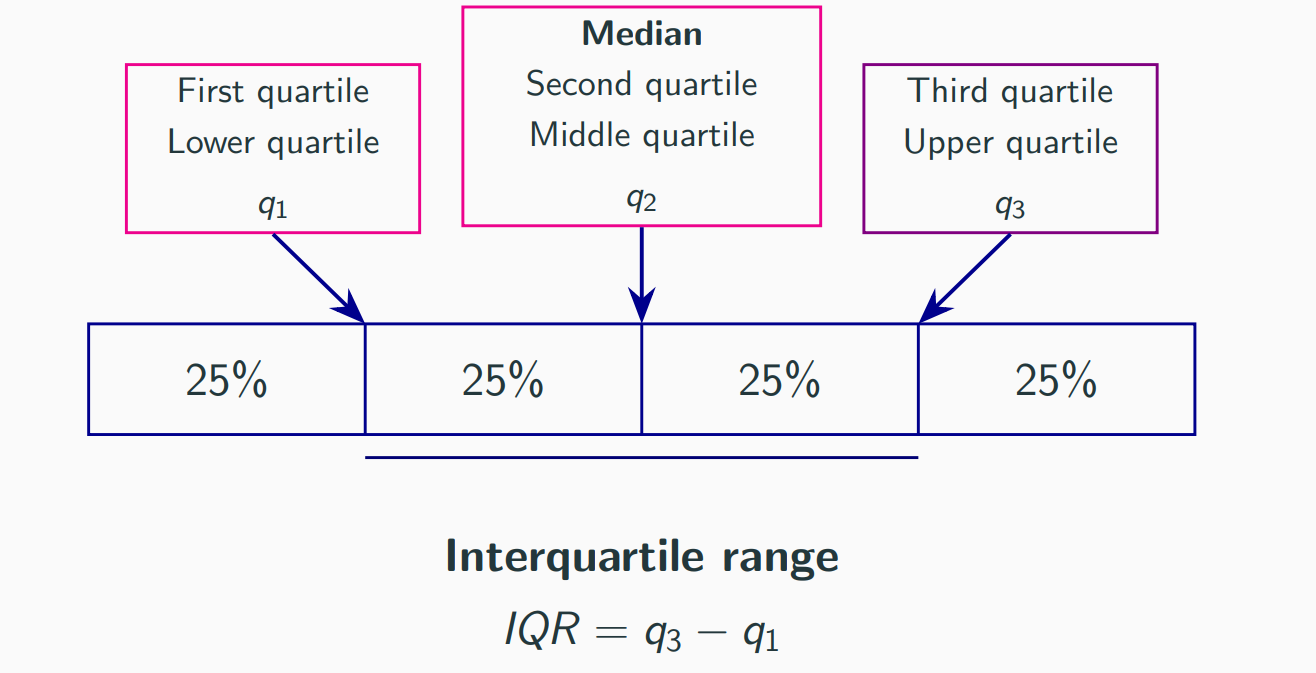
\includegraphics[width=0.6\textwidth]{image_2.png}
  \caption{}
  \label{fig:quartile}
\end{figure}

\section{Ordered statistics}

Let $(X_1,X_2,\dots, X_n)$ be a random sample $(x_1,x_2,\dots,x_n)$ be one its realization. Let's order the values in non-decreasing order and denote as $(x_{(1)}, x_{(2)},\dots, x_{(n)})$ where $x_{(1)} \leq x_{(2)}  \leq \dots \leq x_{(n)}$\\

\textbf{Definition 10.} Let $X_{(k)}$ be a random variable that in each ordered realization $(x_{(1)}, x_{(2)},\dots, x_{(n)})$ of the sample space takes the kth in size value, by $x_{(k)}$, for $k=1,2,\dots,n$. The random variables $X_{(1)}, X_{(2), \dots X_{(n)}}$ are called ordered statistics.

The first ordered statistic is $X_{(1)} = \min\{ X_1, X_2, \dots X_n \}$. The n-th ordered statistic is $X_{(n)} = \max\{ X_1, X_2, \dots X_n \}$\\

\textbf{Definition 11.} The statistic $R=X_{(n)}-X_{(1)}$ is called the range of the sample and each its realization corresponds to the data range.\\

\textbf{Theorem 5:} Let $(X_1, X_2, \dots, X_n)$ be a random sample with size $n\geq2$ from a normal distribution $N(\mu, \sigma^2)$ then

\begin{itemize}
  \item $\overline{X}$ has $N(\mu, \sigma/n)$ distribution
  \item $\frac{(n-1)s^2}{\sigma^2}$ has $\mathcal{X}^2$ distribution with $n-1$ degrees of freedom.
  \item $\overline{X}_n$ and $S^2$ are independent random variable.
  \item The random variable $T$
  \[ T=\frac{\frac{\overline{X}-\mu}{\sigma/\sqrt{n}}}{\sqrt{\frac{(n-1)S^2}{\sigma^2(n-1)}}} = \frac{\overline{X}-\mu}{S}\sqrt{n} \]

  has a student t-distribution with $n-1$ degrees of freedom.
\end{itemize}

\end{document}